\chapter{Development Platform}

To implement the system a hardware platform is needed. The hardware platform can be developed from scratch or be bought as a development board. Developing the hardware platform gives a higher level of customizability, but the development time will be bigger compared to a complete development board. Because of limited time, the system will be developed upon a complete development board. The choice of development board will be based on the requirements, which are listed below.

As previously mentioned, the choice of processor is a DSP, as the DSP has a high performance versus cost. The DSP is also very suitable for signal processing as the CPU architecture usually comes with specialized hardware for tasks such as multiply-accumulate, which can be executed in one instruction. The requirements for the DSP are as follows:

\begin{enumerate}
\item The DSP must have at least two \gls{I2S} ports for interfacing with ADC/DAC.
\item The performance of DSP much be good enough to support least 1024 instructions pr. sample at a sampling rate of 96 kHz.
\end{enumerate}

The development board should also have an integrated audio codec, which ensures the conversion between analog and digital signals. The requirements for the audio codec are as follows:

\begin{enumerate}
\item The sample rate of the audio codec can be adjusted to at least 96 kHz.
\item The audio codec supports a conversion resolution of at least 24-bit.
\end{enumerate}

Further more, the development platform needs accessible external GPIO to allow external interaction with the system, since it is required that the user can change settings on a equalizer. 


\section{Development board TMDX5515EZDSP}

The TMDX5515EZDSP from Spectrum Digital is chosen as the development board. The TMDX5515EZDSP seen in \autoref{fig:TMDX5515EZDSP_overview}. The TMDX5515EZDSP uses a TMS320C5515 DSP from Texas Instruments as the CPU and is interfaced with a TLV320AIC3204 audio codec. Furthermore the development board is interfaced to peripherals such as an OLED screen, two buttons, microSD and a expansion connector with 60 ports. 

\begin{figure}[H]
\centering
\begin{subfigure}[t]{0.47\textwidth}
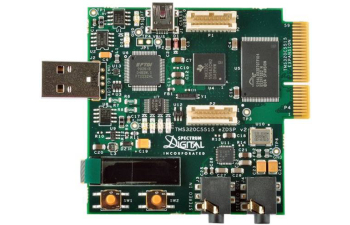
\includegraphics[width=\linewidth]{dsp_board}
	\caption{TMDX5515EZDSP.}
	\label{fig:TMDX5515EZDSP}
\end{subfigure}
\hspace{6mm} 
\begin{subfigure}[t]{0.35\textwidth}
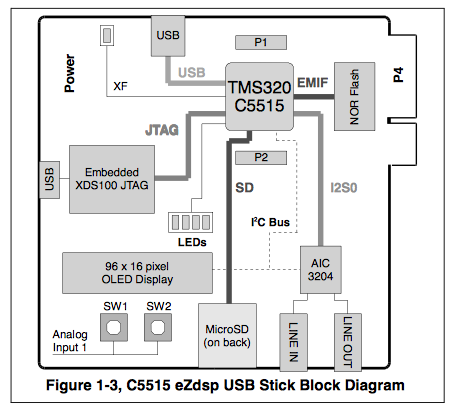
\includegraphics[width=\linewidth]{dsp_blockdiagram}
	\caption{Block diagram overview of the TMDX5515EZDSP.}
	\label{fig:TMDX5515EZDSP_blockdiagram}
\end{subfigure}
\caption{Overview of the TMDX5515EZDSP.}
\label{fig:TMDX5515EZDSP_overview}
\end{figure}

The TMS320C5515 is interfaced to the audio codec through an $\text{I}^2$S bus and $\text{I}^2$C bus. The $\text{I}^2$S bus is used to transmit and receive serial audio data between each unit, while the $\text{I}^2$C is used by the DSP to control the audio codec. According to the datasheet for the TMS320C5515 the input














